\documentclass{beamer}
\usepackage{amsmath}
\usepackage{graphicx}
\usepackage{amssymb}
\usepackage{hyperref}

\title{MATH1061 Week 2 Tutorial}
\date{5 March 2013}

\begin{document}

\frame{\titlepage}

\begin{frame}
\begin{figure}
\centering
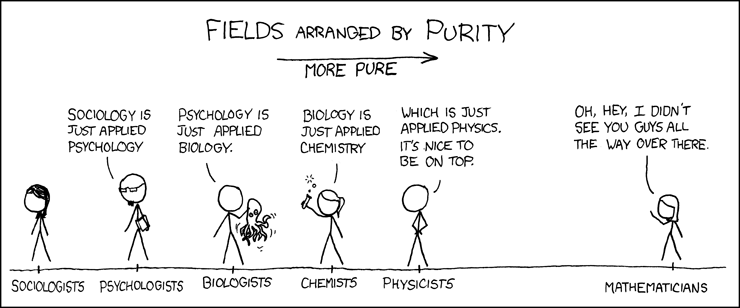
\includegraphics[width=\textwidth]{src/purity.png}
\end{figure}
{\tiny Source: \url{http://xkcd.com/435/}}
\end{frame}

\begin{frame}
\frametitle{Logical Statments}

What is the logical negation of each of these statements?
Which is true - the original statement or its negation? (Check by seeing that
the other one is false)

\begin{enumerate}
\item Our tutorial is in the Priestley building, or you have to submit
your assignments in the Priestley building.
\item If pigs can fly, then Mr. Burns will donate a million dollars to the
local orphanage.\footnote{For this exercise, it is safe to assume that pigs
can't fly. For Mr. Burns, it's not a safe assumption.}
\item If there are Engineering students in the Hawken building, then there will
be a Discrete Maths lecture on Wednesday morning.
\item If the sky is pink, then the sky is blue.
\end{enumerate}

\end{frame}

\begin{frame}
\frametitle{Conditionals}

The following statement is true: ``Jackson brings his umbrella to uni when it's
going to rain". Which of the following is also true?

\begin{enumerate}
\item To rain, it suffices that Jackson brings his umbrella to uni.
\item If it is raining, then Jackson brought his umbrella to uni.
\item If Jackson doesn't have his umbrella, then it's not raining.
\item If it's not going to rain, Jackson won't bring his umbrella.
\item It's necessary that Jackson has his umbrella for it to rain.
\item A rainy forecast causes Jackson to bring his umbrella to uni.
\end{enumerate}

\end{frame}

\end{document}
